\begin{figure}
\centering
\begin{subfigure}{\textwidth}
  \centering
  \includegraphics[width=\columnwidth,page=7]{../images/graphs/condition-dimension.pdf}
  \caption[No visualisation condition enjoyment detailed survey results]{Audience reported enjoyment level for the \textbf{no visualisation} condition.}
  \label{fig:no-visualisation-enjoyment}
\end{subfigure}\\
\begin{subfigure}{\textwidth}
  \centering
  \includegraphics[width=\columnwidth,page=8]{../images/graphs/condition-dimension.pdf}
  \caption[Visualisation condition enjoyment detailed survey results]{Audience-reported enjoyment level for the \textbf{visualisation} condition.}
  \label{fig:visualisation-enjoyment}
\end{subfigure}

\caption[Follow-up user study enjoyment survey responses]{Audience reported enjoyment during the beginning, middle and end of the performance for the no visualisation and visualisation conditions. Line width at each stage indicates proportion of the audience reporting high, medium or low enjoyment, and line colour connecting each section of the performance is determined by the enjoyment level at the \emph{beginning} of the performance.}
\label{fig:follow-up-user-study-condition-enjoyment}
\end{figure}